\documentclass[journal]{IEEEtran}
\usepackage{graphicx}
\usepackage{booktabs}
\usepackage{cite}
\usepackage{url}
\usepackage{siunitx}

\begin{document}

\title{When Does a KV Memory Tier Pay? A First-Order\\Bound, Applied to Preempted KV in Reasoning\\LLM Serving}

\author{Romyull~Islam
\thanks{Manuscript draft, October 2026. R.~Islam is with Kennesaw State University, Kennesaw, GA,
USA (e-mail: mislam22@students.kennesaw.edu).}}% department to be added
\markboth{Draft}{Islam: When Does a KV Memory Tier Pay?}
\maketitle

\begin{abstract}
Host-memory, SSD and CXL tiers for the KV cache now ship in vLLM, LMCache and NVIDIA Dynamo, and
vendors report gains from a few percent to 5.8$\times$. Operators buying memory for KV need to
know where their workload falls. We give a first-order bound: a tier that removes recomputation
raises throughput by about $R/\rho$, where $R$ is the tokens recomputed per token generated and
$\rho$ the cost of a decoded token in units of a recomputed one. Document question answering that
recomputes a 48K-token prompt for 2 output tokens has $R$ in the thousands, and a tier pays many
times over. We apply the bound to the case that reasoning models make common, KV of preempted
requests. Prefill is compute-bound and decode with a full KV cache bandwidth-bound, so $\rho$ is 4
to 30 in today's deployments, while first-come-first-served preemption keeps $R$ below 0.9. A
simulator that follows vLLM's scheduler, calibrated on measured kernels and checked against
LLMServingSim and real vLLM runs, matches the bound within 0.3 points on a production reasoning
trace and best-of-$N$ math workloads over seven deployments: a tier for preempted KV raises
saturation throughput by only 2 to 10\%, by 1.7 to 8\% over a tuned admission limit, leaves goodput
unchanged at usable latency targets, and fits in host DRAM except for offline best-of-$N$ batches.
Two counters, $R$ and $\rho$, tell an operator whether a tier will pay.
\end{abstract}

\section{Introduction}
Memory tiers for the KV cache have become products. vLLM's offloading connector and
LMCache~\cite{lmcache} keep KV in host memory, NVIDIA Dynamo's KV block manager adds SSD and remote
tiers~\cite{dynamo_kvbm}, and CXL memory pools are offered as the next tier~\cite{tang_cxl}. Their
reported value varies widely. In Samsung's evaluation a CXL pool used by LMCache keeps 354K tokens/s
on document question answering where 512\,GB of DRAM alone falls to 61K because KV must be
recomputed, a 5.8$\times$ gain~\cite{samsung_cmmd}; Tang et al.\ report a 30\% larger
batch~\cite{tang_cxl}; and vLLM recomputes preempted requests by default because recomputation is
often faster than swapping~\cite{vllm,infermax}. An operator deciding whether to buy host or CXL
memory for KV has no way to tell which of these a workload will see.

Reasoning models make the question pressing for one use in particular. They generate thousands to
hundreds of thousands of tokens per request with heavy-tailed lengths: on a production reasoning
trace from Qwen-Bailian~\cite{bailian} the median output is 1.7K tokens, the 99th percentile 35K,
and the longest 10\% of requests hold 71\% of the KV byte-seconds. No batch size fits both the
median and the tail, so KV, not compute, limits the batch~\cite{kinetics,infscaling} and requests
that outgrow it are preempted: in our saturation runs 30 to 98\% of requests are preempted, up to
9 times each, and preemption is routine in reasoning RL rollouts~\cite{rollpacker}. vLLM then
recomputes their KV from scratch~\cite{vllm}. Keeping that KV instead is the use that offloading
tiers restore first and the natural use of cheap CXL capacity~\cite{infercept,fastserve,cacheopt}.

We ask two questions. When does a KV memory tier pay, for any workload? And for preempted KV of
reasoning traffic, how much throughput does it add and how much capacity does it need? Two facts
behind the answers are known. Decode costs far more per token than prefill: Sarathi measures 16.7
to 200 times at small batch~\cite{sarathi}, and phase-splitting systems are built on the
gap~\cite{splitwise,distserve}. And InferCept and restore-or-recompute models weigh swapping against
recomputing per request~\cite{infercept,restore_recompute}. What is missing is a workload-level bound
and measurements of its inputs.

This letter contributes (1) the bound $R/\rho$, which places document question answering
($R$ in the thousands) and preempted KV ($R<0.9$) at opposite ends; (2) measurements of $R$,
$\rho$ and the gain for preempted KV on a production reasoning trace and best-of-$N$ math workloads
over seven deployments, with a simulator validated against LLMServingSim and real vLLM runs, showing
a gain of only 2 to 10\%; (3) the tier capacity this needs, which host DRAM already provides; and
(4) the conditions under which a tier for preempted KV would pay.

\section{First-order model}
\label{sec:model}
Let $c_d$ be the GPU time per decoded token in a batch with a full KV cache and $c_r$ the time per
recomputed token. If preemption recomputes $R$ tokens per generated token, the recompute share of
GPU time is $w = R c_r / (c_d + R c_r) = R/(\rho + R)$ with $\rho = c_d/c_r$, and a tier that
removes all recomputation raises throughput by $w/(1-w) \approx R/\rho$.

$\rho$ is large. A decode step reads the weights and every running request's KV from HBM, and
with the KV cache full it reads all of it, so $c_d \approx (W + K)/(B \cdot \mathrm{BW})$ for
weights $W$, KV $K$ and batch $B$. Recompute is a prefill: about $2P$ FLOPs per token plus
attention, at high utilization. For a 70B model on 8 H100 GPUs $\rho$ is 6 to 15. $R$ is small
because vLLM puts a preempted request at the head of the waiting queue: it resumes as soon as
memory frees up, so most requests are recomputed at most once. Even with 90\% of requests
preempted, $R$ stays below 0.9 in our runs. The gain is thus bounded by about $0.9/\rho$.

The bound explains the published gains. Samsung's benchmark asks 2-token questions about
48K-token documents~\cite{samsung_cmmd}, so every miss recomputes 24,000 tokens per generated token
and a tier that avoids it multiplies throughput. Tang et al.\ report a 30\% larger batch with a
CXL KV store than with full recomputation~\cite{tang_cxl}; that is also reuse of shared prefixes
across requests, with $R$ of many tokens per generated token, not preemption. A dynamical model of evict-and-restart finds throughput losses as large as
50\%~\cite{congestion} in a worst case of identical request lengths and synchronized evictions;
the same work shows that length heterogeneity stabilizes the system, and reasoning lengths are
heavy-tailed.

\section{Methodology}
\label{sec:method}
\textbf{Simulator.} A step-level simulator follows vLLM V1's scheduler: running requests are served
in admission order, the last one is preempted when a block is missing, and preempted requests
resume first; freed blocks stay in the prefix cache until reused. Tier policies: swap on
preemption, and write-through with LRU eviction as in vLLM's CPU offloading connector.

\textbf{Step time.} A roofline whose efficiencies are fitted to Vidur's measured kernel
profiles~\cite{vidur}: whole-layer error 4 to 10\% median on H100 (Llama-2-70B, held-out
CodeLlama-34B) and 4 to 7\% on A100 (Llama-3-70B, held-out Llama-3-8B, contexts to 16K). Prefill
attention uses FlashAttention-3 efficiency~\cite{fa3} or, as a pessimistic case that makes
recompute dearer, the measured FlashAttention-2 curve.

\textbf{Validation.} Against LLMServingSim 2.0~\cite{llmservingsim2}, an independent port of
vLLM's scheduler with its own GPU profiles, on 64 requests with 10K to 30K-token outputs:
preemptions 50 vs 50, recomputed tokens within 0.3\%, per-request finish times correlated at
0.9999. Against real vLLM 0.31 (Qwen2.5-0.5B, KV fixed at 4,096 blocks, 300 requests with
Bailian lengths): 297 vs 277 preemptions and 111K vs 118K recomputed tokens. With a reasoning model
(DeepSeek-R1-Distill-Qwen-1.5B on an RTX 4500 Ada, about 2\,GB of KV, 400 requests of the Bailian
trace with outputs up to 32K tokens), vLLM preempted 275 times and recomputed 569K tokens; the
simulator predicts 270 and 574K.

\textbf{Workloads and deployments.} The Bailian reasoning trace (10,812 requests, real arrivals)
and best-of-1, 16 and 64 groups of MathArena AIME 2025 outputs from the model with the matching
architecture~\cite{matharena}. Llama-70B on 8 H100, H200 and B200; QwQ-32B on 2 and 4 H100;
Qwen3-235B FP8 on 8 H100; DeepSeek-R1 FP8 on 8 H200, whose replicated MLA latent holds only 0.56M
tokens. vLLM defaults: block 16, up to 1,024 running requests, 8,192 tokens per step.

\section{Results}
\label{sec:results}

\begin{figure}[t]
\centering
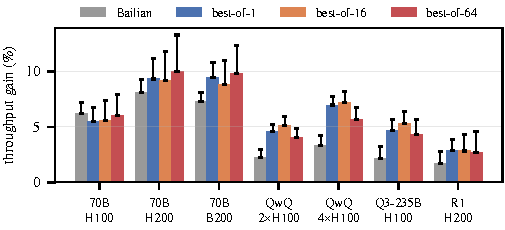
\includegraphics[width=\columnwidth]{fig_gain.pdf}
\caption{Saturation throughput gain of keeping preempted KV (unlimited tier) over recompute; bars
use FlashAttention-3 efficiency, whiskers the FlashAttention-2 calibration.}
\label{fig:gain}
\end{figure}

\textbf{Saturation.} With every request submitted at once, the regime with the most preemption,
keeping preempted KV raises throughput by 2 to 10\% (median 5.5\%) and by at most 13\% with the
pessimistic prefill calibration (Fig.~\ref{fig:gain}), although 30 to 98\% of requests are
preempted, up to 9 times each. Fig.~\ref{fig:model} places every run in the model's plane: the
simulated gains match $w/(1-w)$ with correlation 0.997 and a mean error of 0.3 points. The gain is
largest for 70B on H200 and B200, whose larger batches make decode cheaper per token, and smallest
for DeepSeek-R1.

\begin{figure}[t]
\centering
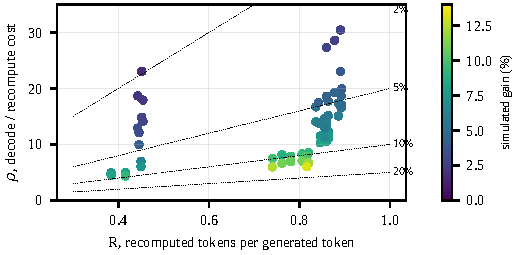
\includegraphics[width=\columnwidth]{fig_model.pdf}
\caption{Every saturation run in the model's plane; dotted lines are constant gain $R/\rho$.}
\label{fig:model}
\end{figure}

\textbf{Admission tuning.} Lowering vLLM's running-request limit from 1,024 to 96 to 192 recovers
up to 6\% by itself; over the best-tuned recompute baseline an unlimited tier adds 1.7 to 5.9\%
with BF16 KV and 5 to 8\% with FP8 KV, the most favorable case we found, because FP8 halves the KV
read per decode step and so halves $\rho$.

\textbf{Online load.} Below saturation the gain is zero. Goodput, the highest load that keeps the
99th-percentile time to first token under 10 or 60\,s, is unchanged in 19 of 20 cases. The tier
cuts tail latency only where the queue is already minutes long.

\begin{figure}[t]
\centering
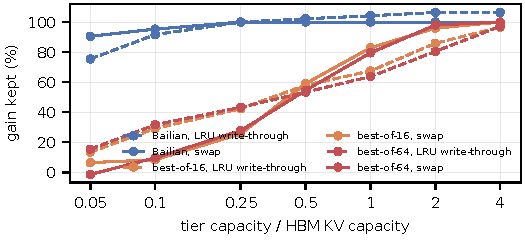
\includegraphics[width=\columnwidth]{fig_capacity.pdf}
\caption{Share of the unlimited tier's gain kept versus tier capacity (median over 70B on H100 and
H200, QwQ-32B and DeepSeek-R1).}
\label{fig:cap}
\end{figure}

\textbf{Capacity.} For production arrivals a tier of 0.1 to 0.25 times the HBM KV capacity keeps
93 to 100\% of the gain (Fig.~\ref{fig:cap}); online it peaks at 62\,GB. Only offline best-of-$N$
batches submitted at once need 1 to 2 times the HBM KV with swap and 2 to 4 times with LRU
write-through, up to 3.4\,TB for 70B on 8 H200 GPUs, against 2\,TB of DRAM in a DGX node. Pooling
eight nodes' tiers saves 49 to 64\% of capacity, but the pooled peak (at most 1.3\,TB) is far below
the nodes' combined DRAM, so CXL capacity is not needed.

\textbf{Real system.} On real vLLM with the 0.5B model, removing the memory pressure altogether
raised throughput by only 5.9\%, and vLLM's native CPU offloading tier lowered it by 3.9\%: it
reloaded 41\% of the preempted KV and paid for writing all KV through to the CPU. With the
reasoning model the offloading tier removed 43\% of the recomputed tokens. Measured directly on that
GPU, a decoded token cost 0.68, 2.7 and 5.5\,ms and a recomputed one 30, 36 and \SI{43}{\micro\second}
at 2K, 8K and 16K tokens of context: $\rho$ = 23, 77 and 128, larger than in our deployments because
the small KV budget forces batches of 17, 4 and 2. Here $R$ was 0.43, so $R/\rho$ bounds the gain at
2\% even at 2K tokens.

\section{When does a tier pay?}
The bound points to three ways a KV tier becomes worth its memory. First, cheaper
decode lowers $\rho$: FP8 or INT4 KV halves or quarters the bytes read per decode step, and larger
HBM allows larger batches; with FP8 KV our gain over tuned admission rises to 5 to 8\%, and on H200
and B200 the gain is larger than on H100. Second, schedulers that preempt on purpose raise $R$: a
latency-oriented scheduler that time-slices long requests, as in skip-join multi-level
feedback~\cite{fastserve}, recomputes the same context many times, so $R$ can exceed 1 and the tier
pays roughly in proportion. Third, workloads whose prompts dwarf their outputs raise $R$: document
question answering~\cite{samsung_cmmd}, and agents whose context is evicted while they wait for a
tool and is recomputed for a short next turn~\cite{efficientagent,unison}. Under first-come-first-served admission neither holds, over-admission
rather than missing capacity causes the recomputation, and a better admission limit removes part of
it at no cost. Operators can check their own deployment with two numbers: $R$ from the scheduler's
counters and $\rho$ from a short microbenchmark like the one above.

\section{Discussion}
\textbf{Limitations.} The step-time model is calibrated on 4K to 16K-token profiles and extrapolated
physically beyond; MLA and MoE timings are not validated against measurements; prompts shared
across requests are not modeled.

\textbf{Related work.} Prior work characterizes the memory wall of reasoning~\cite{kinetics,infscaling}, tiers decoding
KV with sparse attention~\cite{oasiskv,notallthoughts}, manages memory for tree
search~\cite{fasttts}, and models preemption from length distributions~\cite{congestion} or
measures it in RL rollouts~\cite{rollpacker}, and robust admission sets KV reservations under
length uncertainty~\cite{robustkv}. EfficientAgent sizes a host tier for paused agents'
KV~\cite{efficientagent}. We add a workload-level bound on what keeping preempted KV can gain,
measurements of its inputs for reasoning traffic, and its validation.

\section{Conclusion}
For reasoning and test-time-scaling workloads, keeping preempted KV in host DRAM or CXL memory is
worth 2 to 10\% of saturation throughput and nothing at usable latency, because a recomputed token
costs a fourth to a thirtieth of a decoded one and first-come-first-served preemption recomputes less
than one token per token generated.

\bibliographystyle{IEEEtran}
\bibliography{p1}

\end{document}
